\documentclass[10pt,a4paper]{article}

\usepackage[margin=1.8cm]{geometry}
\usepackage{amsmath}
\usepackage{array}
\usepackage{booktabs}
\usepackage{graphicx}
\usepackage{tabularx}
\usepackage[hidelinks]{hyperref}
\graphicspath{{./}{report/}}

\setlength{\parindent}{0pt}
\setlength{\parskip}{4pt}
\setlength{\tabcolsep}{3pt}
\renewcommand{\arraystretch}{1.12}
\newcolumntype{Y}{>{\raggedright\arraybackslash}X}

\begin{document}

\section{Task 0: Model Hub warm-up}

\begin{table}[ht]
\centering
\footnotesize
\begin{tabularx}{\textwidth}{@{}p{2.4cm}p{2.3cm}Yp{2.0cm}Yp{2.3cm}@{}}
\toprule
Model ID & Training tokens or steps & Architecture & Trainable parameters & Training data & Sources \\
\midrule
\texttt{allenai/OLMo-1B}
& 3 trillion tokens
& 16 layers; hidden size 2,048; 16 attention heads
& Approximately 1.2B
& Dolma v1.5: web content, academic publications, code, books, and encyclopedic material
& \href{https://huggingface.co/allenai/OLMo-1B}{Model card};
  \href{https://huggingface.co/allenai/OLMo-1B/blob/main/config.json}{config.json};
  \href{https://huggingface.co/datasets/allenai/dolma}{Dolma card} \\
\addlinespace
\texttt{HuggingFaceTB/\allowbreak SmolLM2-360M}
& 4 trillion tokens
& 32 layers; hidden size 960; 15 query heads and 5 key/value heads
& Approximately 362M
& FineWeb-Edu, DCLM, The Stack, and additional filtered datasets curated by Hugging Face
& \href{https://huggingface.co/HuggingFaceTB/SmolLM2-360M}{Model card};
  \href{https://huggingface.co/HuggingFaceTB/SmolLM2-360M/blob/main/config.json}{config.json};
  \href{https://arxiv.org/abs/2502.02737}{report} \\
\addlinespace
\texttt{Qwen/\allowbreak Qwen2.5-0.5B}
& 18 trillion tokens for the Qwen2.5 series; no separate 0.5B count is published
& 24 layers; hidden size 896; grouped-query attention with 14 query heads and 2 key/value heads
& 0.49B total; 0.36B excluding embeddings
& Filtered multilingual data emphasizing knowledge, mathematics, and code, including synthetic data; the exact corpus list is not disclosed
& \href{https://huggingface.co/Qwen/Qwen2.5-0.5B}{Model card};
  \href{https://huggingface.co/Qwen/Qwen2.5-0.5B/blob/main/config.json}{config.json};
  \href{https://arxiv.org/abs/2412.15115}{report} \\
\bottomrule
\end{tabularx}
\caption{Model IDs for the Hub warm-up exercise.}
\label{tab:model-hub-warmup}
\end{table}

The model cards provide training-token totals and summarized model details.
The configuration files provide layer counts, hidden dimensions, and
attention-head configurations. Dataset cards and technical reports provide
the training-data descriptions. Qwen's report describes data categories and
curation methods, but does not publish a complete list of source corpora.

\clearpage
\section{Task 1: Tokenization}

Two byte-level BPE tokenizers were trained on the same 500-million-character
CLIMBMix sample, with vocabularies of 8,192 and 32,768 tokens. BPE begins with
bytes and repeatedly replaces the most frequent adjacent pair with a new
symbol. Unlike a word vocabulary it can represent unseen words, while its
learned multi-byte units produce shorter sequences than character-level
tokenization.

\begin{table}[ht]
\centering
\small
\begin{tabular}{@{}lrrrrr@{}}
\toprule
& Characters & \multicolumn{2}{c}{8,192} & \multicolumn{2}{c}{32,768} \\
Sample & & Tokens & Tokens/char & Tokens & Tokens/char \\
\midrule
English & 87 & 17 & 0.1954 & 15 & 0.1724 \\
Numbers & 64 & 32 & 0.5000 & 31 & 0.4844 \\
Python & 64 & 32 & 0.5000 & 26 & 0.4062 \\
Dutch & 67 & 28 & 0.4179 & 23 & 0.3433 \\
\bottomrule
\end{tabular}
\caption{Token counts on fixed held-out examples. Lower tokens/character is better.}
\label{tab:tokenizer-compression}
\end{table}

\begin{minipage}[t]{0.47\textwidth}
\textbf{Merge example.} For the original corpus
\texttt{banana bandana banana}, one possible tie-breaking order is:
\texttt{a+n $\rightarrow$ an} [6],
\texttt{b+an $\rightarrow$ ban} [3],
\texttt{an+a $\rightarrow$ ana} [3], and
\texttt{ban+ana $\rightarrow$ banana} [2]. The bracketed value is the pair
count when that merge is made.

\begin{verbatim}
banana [2]
|-- ban [3]
|   |-- b
|   `-- an [6] = a + n
`-- ana [3]
    |-- an [6]
    `-- a
\end{verbatim}

The 32K tokenizer reduced the English sequence by two tokens (11.8\%) because
it learned whole units such as \texttt{learns} and \texttt{matters}; the 8K
model split these into \texttt{lear+ns} and \texttt{matter+s}.
\end{minipage}\hfill
\begin{minipage}[t]{0.50\textwidth}
\textbf{Downstream trade-off.} A larger vocabulary shortens sequences, but
the embedding and output matrices grow linearly with vocabulary size. It also
increases the softmax denominator: every prediction must distribute
probability over more classes. Rare merged tokens receive fewer updates, so
their representations can be less reliable. A smaller vocabulary reverses
these trade-offs but requires more transformer steps for the same text.

\textbf{Artifacts.} Numbers remained fragmented into one- or two-digit units,
for example \texttt{20|26|-|09|17}; this follows nanochat's numeric split
pattern. Code improved most when moving to 32K (32 to 26 tokens), which learned
pieces such as \texttt{def}, \texttt{ cube}, and \texttt{(n}, while identifiers
and punctuation still split around \texttt{\_}, brackets, and spaces. Dutch
also improved, but remained more fragmented than English
(\texttt{tre|in}, \texttt{re|kt}, \texttt{ach|t}), consistent with less useful
merge coverage. Byte-level fallback prevented unknown tokens in every sample.
\end{minipage}

\clearpage
\section{Task 2: Pre-Training}

\subsection*{Depth and run configuration}

The model was pre-trained on CLIMBMix with \texttt{--depth=2}. Depth directly
sets the number of transformer blocks. Nanochat first computes a base width of
$64d$, rounds it to a multiple of the 128-dimensional attention head, and sets
the number of heads to width divided by 128. Thus $d=2$ gives width 128 and one
query/key-value head. The same dial also determines the parameter count used
for the training horizon. Nanochat then derives the token batch from its batch
scaling rule and adjusts learning rates and weight decay for that batch and
width. It uses 40 warmup steps followed by a constant phase and a linear
warmdown over the final 65\% of training. The run used full-context attention
because the local Windows CUDA
installation used PyTorch SDPA rather than Flash Attention 3.

\begin{table}[ht]
\centering
\small
\begin{tabular}{@{}lr@{\qquad}lr@{}}
\toprule
Transformer layers & 2 & Context length & 2,048 \\
Attention heads & 1 & Vocabulary & 32,768 \\
Embedding width & 128 & Trainable parameters & 12,976,170 \\
Scaling parameters & 4,587,532 & Token batch & 131,072 \\
Training steps & 420 & Training tokens & 55,050,240 \\
\bottomrule
\end{tabular}
\caption{Depth-2 model and training configuration. Training took 36.1 minutes.}
\label{tab:task2-config}
\end{table}

A single complexity dial makes model-size sweeps simple and reproducible: a
depth can be selected without separately finding a compatible width, head
count, batch size, and schedule. Its limitation is that these coupled rules
may not be optimal for a particular dataset, hardware budget, or architectural
choice. Independent tuning could find a better width/depth balance or training
horizon, at the cost of a much larger search space.

\subsection*{Scaling-law comparison}

The Chinchilla rule of thumb is approximately 20 training tokens per parameter
\href{https://arxiv.org/abs/2203.15556}{(Hoffmann et al., 2022)}. Using all
12,976,170 trainable parameters gives
\[
D_{\mathrm{Chinchilla}} \approx 20N = 259,523,400\ \text{tokens}.
\]
Nanochat instead applies its default ratio of 12 to 4,587,532 ``scaling
parameters'' (transformer matrices plus the language-model head), excluding
the embedding and value-embedding tables. Its target is therefore 55,050,384
tokens; rounding to complete 131,072-token batches produced 55,050,240 tokens.
This is 21.2\% of the $20N$ estimate, so the model is under-trained relative to
the Chinchilla heuristic. Under-training means using fewer tokens than the
compute-optimal allocation for a model size; over-training means spending more
tokens after a smaller model would have been the more compute-efficient choice.
The comparison is approximate because nanochat deliberately counts parameters
differently.

\subsection*{Bits-per-byte analysis}

\begin{figure}[htbp]
\centering
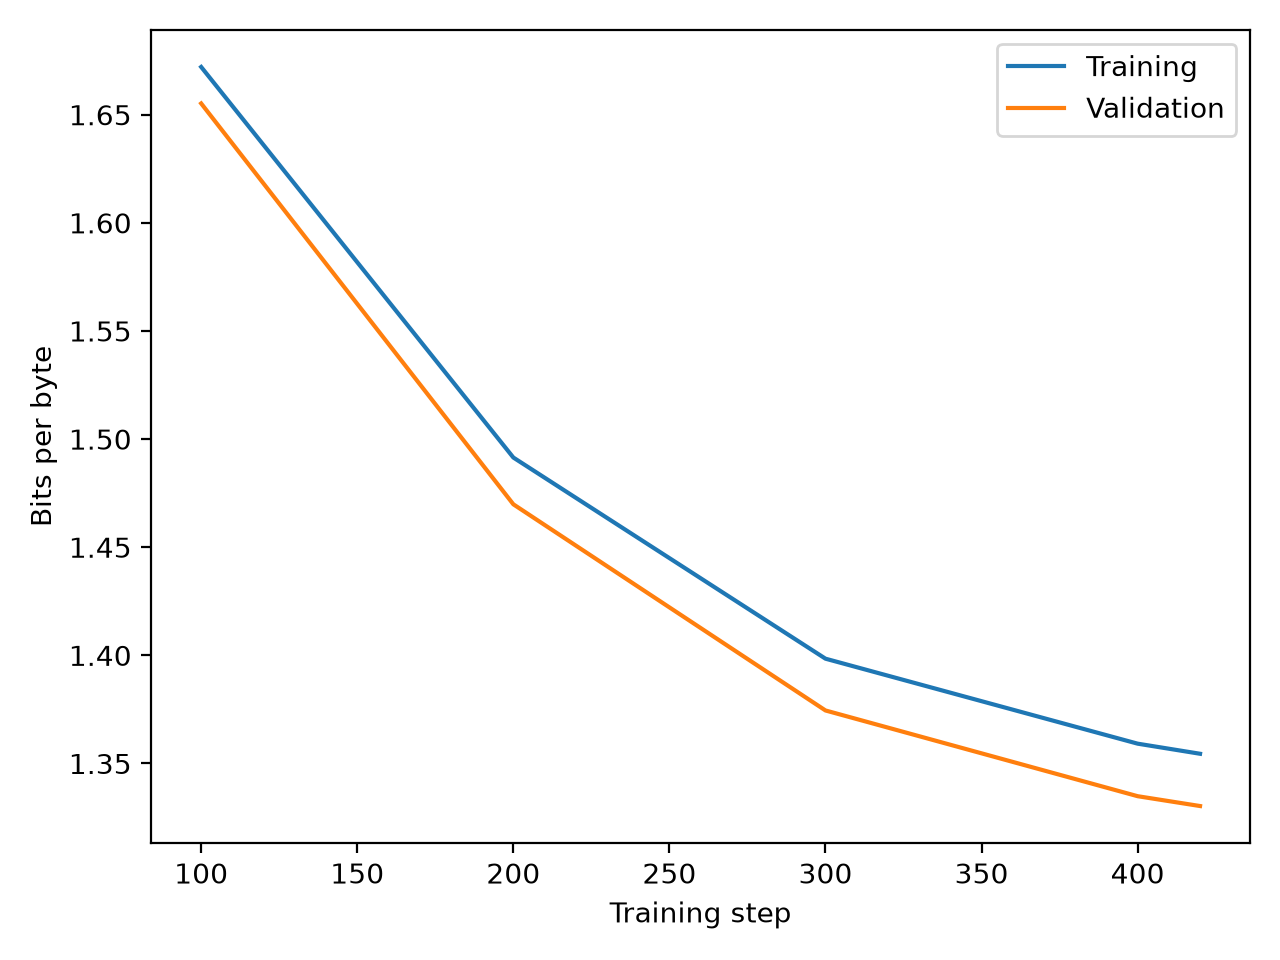
\includegraphics[width=0.58\textwidth]{task2_bpb.png}
\caption{Training and validation bpb, re-evaluated on fixed 1,048,576-token
splits at each saved checkpoint. Lower is better.}
\label{fig:task2-bpb}
\end{figure}

Both curves decrease quickly and then flatten. Validation bpb improves from
1.655 at step 100 to 1.470, 1.374, 1.335, and 1.330 at steps 200, 300, 400,
and 420. The gain per 100 steps falls from 0.185 to 0.095 and then 0.040, so
flattening is visible after roughly step 300 and is strongest near step 400.
Training bpb follows the same shape, falling from 1.672 to 1.354. Validation
bpb remains about 0.02 lower than the fixed training slice. This small reversed
gap gives no evidence of overfitting; it more likely reflects a slightly easier
validation shard or sampling variation between the two fixed slices.

\subsection*{Qualitative inspection}

Five greedy 16-token continuations were sampled from the final base checkpoint
with a beginning-of-sequence token and plain text only, without a system prompt
or chat template:

\begin{enumerate}
\small
\item \textbf{The capital of France is} --- ``a world of France. The world of
France is a world of France and France''
\item \textbf{The chemical symbol of gold is} --- ``a chemical symbol of gold
and gold. The gold is a chemical symbol of gold''
\item \textbf{If yesterday was Friday, then tomorrow will be} --- ``a week,
and the day will be the first week. The week will be''
\item \textbf{The opposite of hot is} --- ``the most common cause of the most
common cause of the most common cause of the''
\item \textbf{The planets of the solar system are:} --- ``the sun's sun's
sun's sun's sun's sun's sun's sun''
\end{enumerate}

The model has learned local English syntax and topical associations: the
outputs stay near words such as France, gold, week, and sun. It has not learned
reliable facts or simple temporal reasoning, and several outputs collapse into
repetition. This is expected from a two-layer, 13-million-parameter base model
trained for only 55 million tokens. It has also received next-token
pre-training only, so it has not been taught instruction following or dialogue
behaviour. The final saved model is \texttt{model\_000420.pt} under the
\texttt{task2-d2} checkpoint tag.

\end{document}
